
\documentclass[11pt,a4paper]{article}
\usepackage[utf8]{inputenc}
%\usepackage[icelandic]{babel}
%\usepackage[T1]{fontenc}
\usepackage{amsmath}
\usepackage{amsfonts}
\usepackage{amssymb}
%\usepackage{graphicx}
%\author{Arnar Ingi Halldórsson}
%\title{Linear Motion}


%\documentclass{article}
\usepackage{graphicx}
\graphicspath{ {myndir/} }
\usepackage[T1]{fontenc} 
\usepackage[english]{babel}

\usepackage[utf8]{inputenc} 
\usepackage{graphics}
%\usepackage[pdftex]{graphicx}

\usepackage{caption}
\usepackage{subcaption}
\usepackage[top=2in, bottom=1.5in, left=1in, right=1in]{geometry}
%\usepackage{titling}

%\setlength{\droptitle}{-10em}
   
\title{Assignment 1 \\ T-509-RAFT \\ Electronics} % Title

\author{Arnar Ingi Halldórsson \\ Hjörleifur G. Bergsteinsson \\ Snorri Stefánsson} % Author name
\begin{document}

\maketitle % Insert the title, author and date

\begin{tabular}{lr}
Due date: 22.02.2015 \\
Teachers:\qquad Slawomir Koziel\\ % Instructor/supervisor
\qquad \qquad \qquad Adrian Bekasiewicz
\end{tabular}

\setlength\parindent{0pt} % Removes all indentation from paragraphs

\renewcommand{\labelenumi}{\alph{enumi}.} % Make numbering in the enumerate environment by letter rather than number (e.g. section 6)

\section*{Introduction}

The purpose of the assignment is to determine performance parameters of the operational amplifiers as well as the simulation and design of a half-wave rectifier using $NI \, Multisim$

\section*{Task 1: Perfomance Parameters of Op Amp}

\begin{enumerate}
  \item[1.]
  The circuit diagram in figure 1 was simulated in $MultiSim$ to find the slew-rate (SR) of a 741 op amp.\\
    \begin{minipage}{\linewidth}
      \centering       
       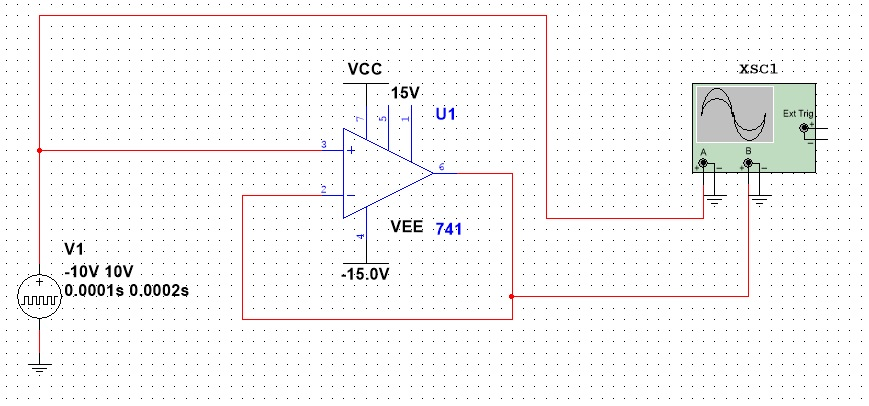
\includegraphics[width=10cm]{Task1-1Circuit}\\
     \captionof{figure}{The circuit in Task 1.1} 
    \end{minipage}\\
\pagebreak
\pagebreak

Measurements from the Oscilloscope can be shown in figure 2. The diagram shows the effect of the slew rate limiting the output and its rectangular waveform.\\
	
    \begin{minipage}{\linewidth}
      \centering       
       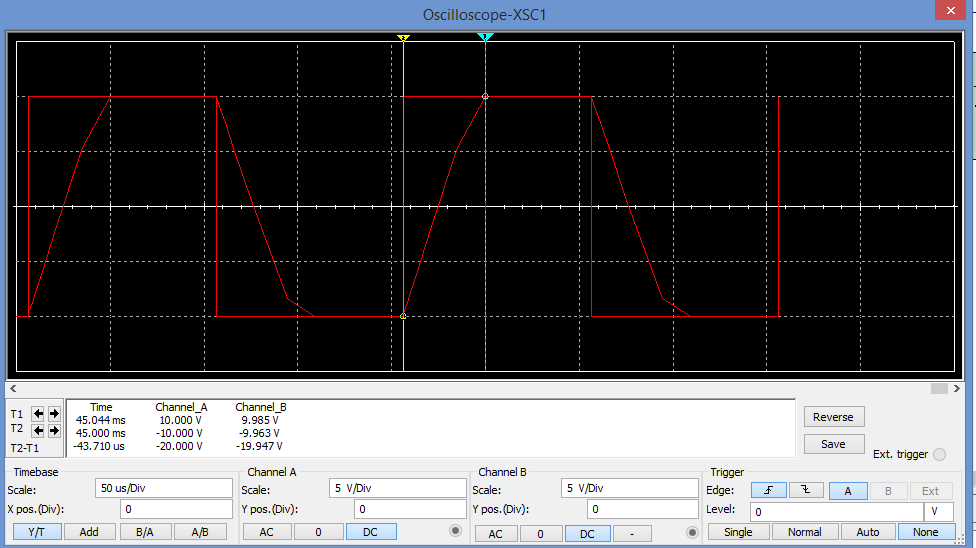
\includegraphics[width=10cm]{Task1-1-Oscilloscope}\\
      \captionof{figure}{Data from the oscilloscope} 
    \end{minipage}
$$ \text{SR} = \dfrac{dv_{o}}{dt}|_{max} = \dfrac{-19.947 \ V}{-43.719\ \mu s} = 0.456\ \frac{V}{\mu s} $$
  \item[2.]
  The circuit diagram shown below in figure 3 was simulated with an AC analysis to determine the gain-bandwidth product (GBW) of the op amp.  
  
      \begin{minipage}{\linewidth}
      \centering
        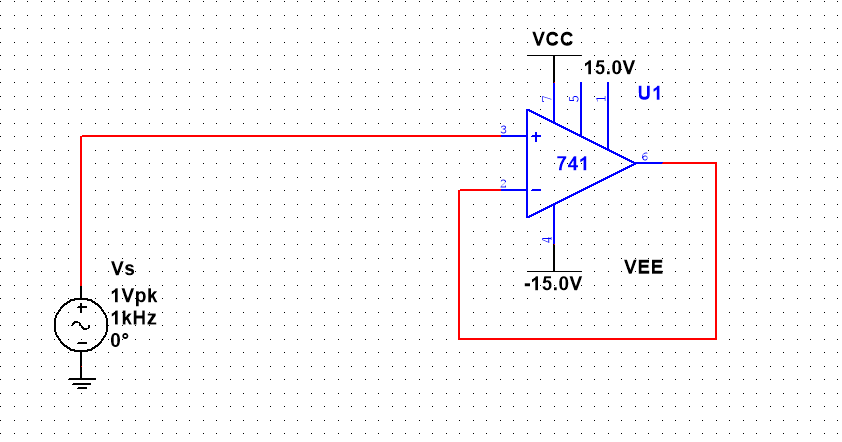
\includegraphics[width=10cm]{Task1-2-Circuit}\\
    \captionof{figure}{Circuit in Task 1.2} 
    \end{minipage}
    
   The measurements from the AC analysis of the circuit can be observed in figure 4. By finding the $f_H$ the gain-bandwidth product can be calculated.
    $$ BW \simeq f_{H} $$
    $$ GB = |A_{G}|BW $$
    
    This is a voltage follower so it has unity gain, $|A_{G}| = 1$. 
    $$ GB = BW $$
    
    The $f_{H}$ is 995.486 kHz as seen in figure 4. Hence the gain-bandwidth product is:
    $$ GB = 995.486 \ kHz$$
    
    \begin{minipage}{\linewidth}
      \centering
        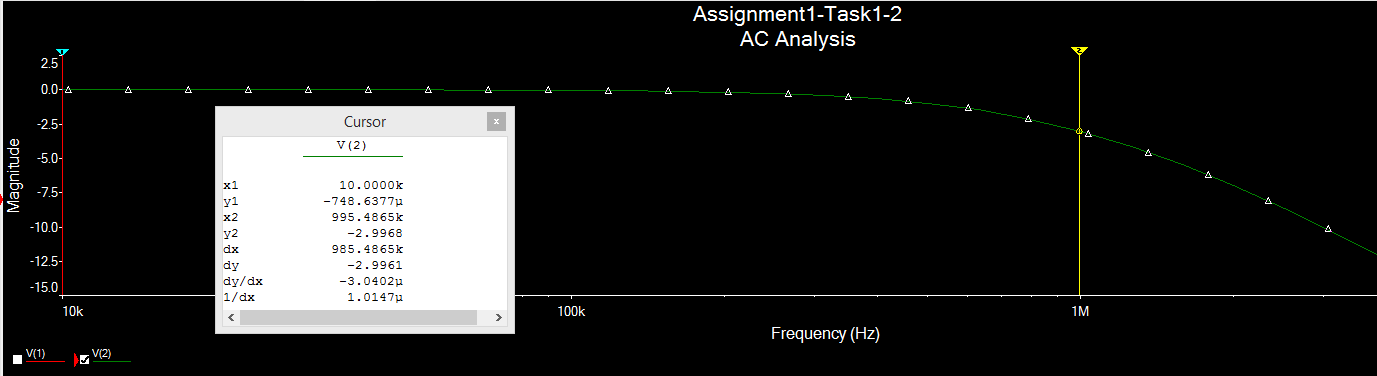
\includegraphics[width=15cm]{Task1-2-ACAnalysis}\\
    \captionof{figure}{AC analysis of the circuit in figure 3 }     
    \end{minipage}
  %     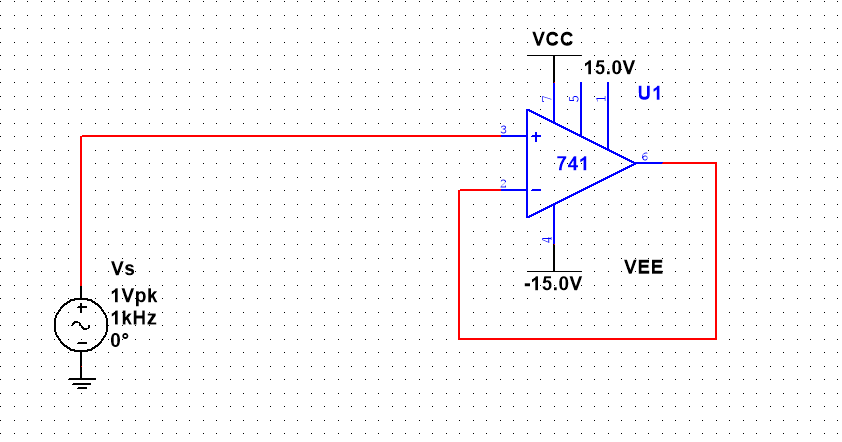
\includegraphics[width=10cm]{Task1-2-Circuit}\\
    % 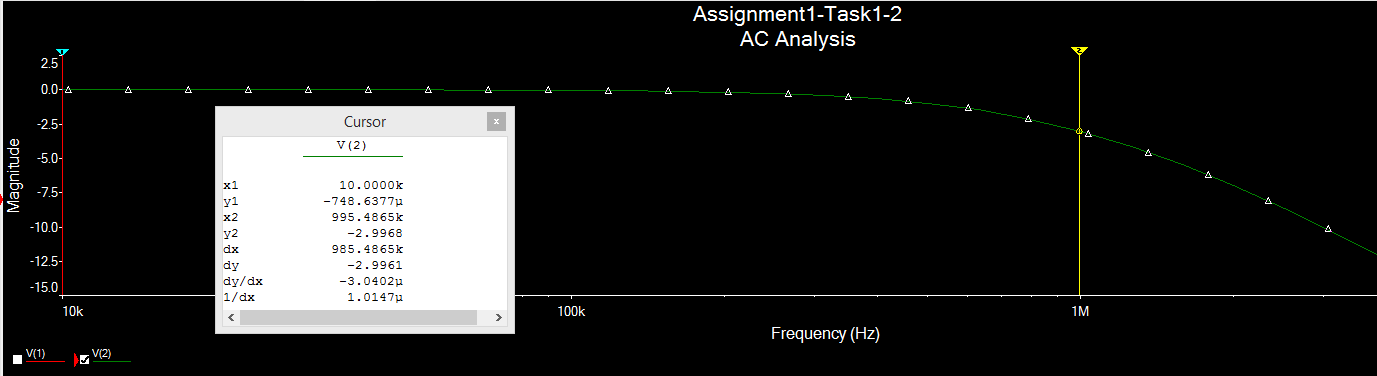
\includegraphics[width=10cm]{Task1-2-ACAnalysis}\\
  \item[3.]
  
  
  The circuit below was simulated in $MultiSim$ to determine the DC differential gain $A_{d}$ and the input offset voltage $V_{OS}$ of the op amp.
  
      \begin{minipage}{\linewidth}
      \centering
      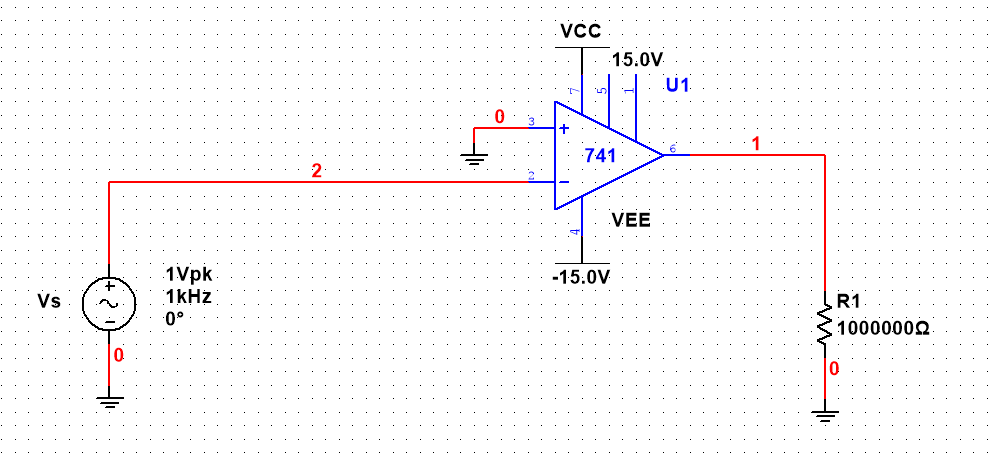
\includegraphics[width=10cm]{Task1-3-Circuit}\\
    \captionof{figure}{The circuit diagram used in task 3.1}   
    \end{minipage}
    
In figure 6 the result of the DC analysis of the circuit in figure 5 can be observed. Hence the DC differential gain is:
$$A_{d} = 206.505\ \frac{V}{mV} $$    
    
    
        \begin{minipage}{\linewidth}
      \centering
      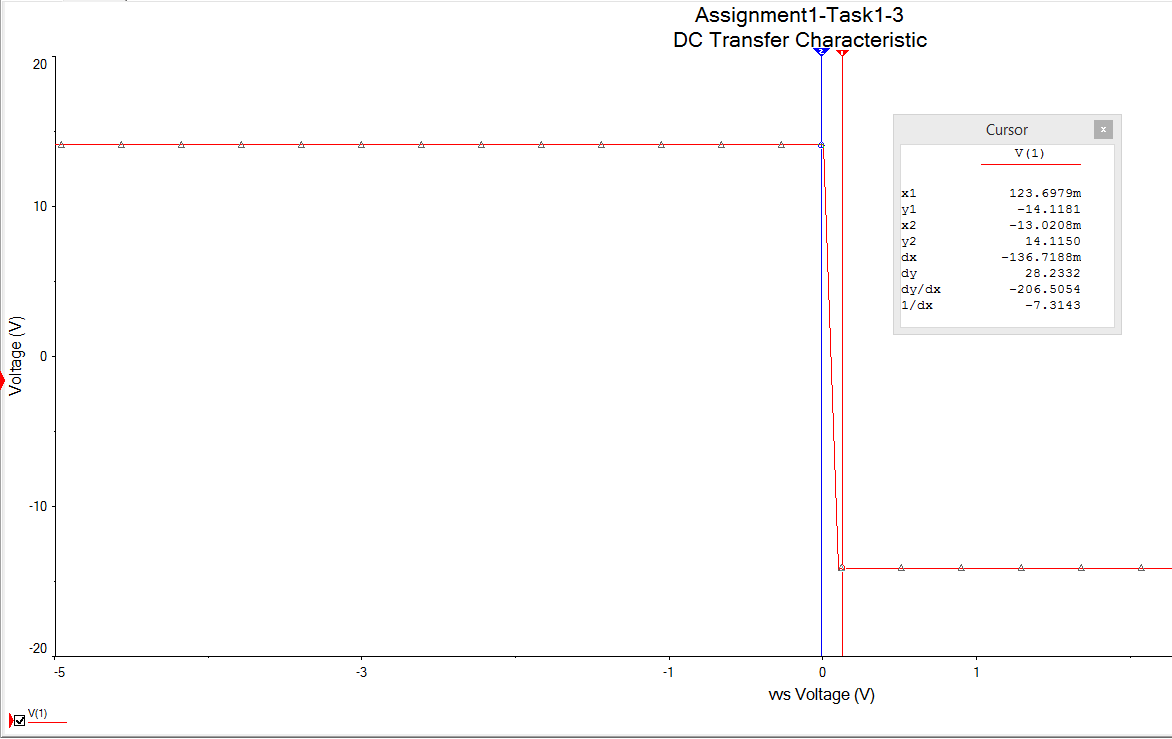
\includegraphics[width=10cm]{Task1-3-DCAnalysis}\\
    \captionof{figure}{DC analysis from circuit in figure 5}    
    \end{minipage}\\   
    
Figure 7 shows the result of the DC analysis. The offset voltage can be determined to be:
$$ V_{OS} = 1.147\ mV $$\\
    
    
\begin{minipage}{\linewidth}
  \centering
    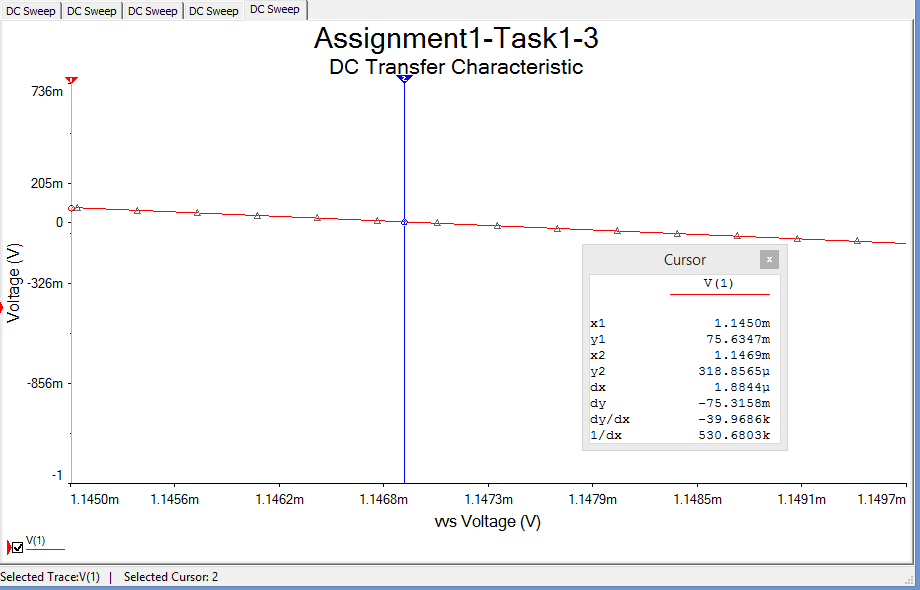
\includegraphics[width=10cm]{Task1-3-Vos}\\
    \captionof{figure}{A closer look of the DC analysis done in figure 6 that allows the offset voltage to be determined}    
    \end{minipage}\\
    
    \pagebreak
 \item[4.]
 

The difference between theoretical and simulated values of the $\mu A741$ op amp can be \\observed in table 1.\\

\begin{minipage}{\linewidth}

\begin{center}
  \begin{tabular}{r l r l r l}
	\multicolumn{2}{c}{$\mu$A741 op-Amp} &   
  \multicolumn{2}{c}{DataSheet} &
  \multicolumn{2}{c}{Simulation}\\
  \hline
  \vspace{0.2em}
  Slew Rate & [$SR$] & 0.5 & $ [\frac{V}{\mu s}]$ & 0.456& $      [\frac{V}{\mu s}]$ \\
  	\vspace{0.2em}
  Gain-Bandwidth & [$GBW$]& 1 &$ [MHz]$  & 995.487 &$ [kHz]$ \\
  	\vspace{0.2em}
  DC Differential Gain &[$A_{d}$] & 200& $[\frac{V}{mV}]$ & 206.505& $[\frac{V}{mV}]$ \\
  	\vspace{0.2em}
  Input Offset Voltage &[$V_{os}$] & 5& $[mV]$& 1.147& $[mV]$ \\
    \end{tabular}
    \captionof{table}{Theoretical and simulated values of $\mu$A741 op amp}
\end{center}
\end{minipage}
\end{enumerate}

\section*{Task 2: Frequency Response of Inverting Amplifier}

\begin{enumerate}
  \item[1.]
  
  In figure 8 shown below the inverting amplifier is simulated in $MultiSim$. The task was to determine the 3 dB corner frequency of the op amp with an AC analysis.\\
  \begin{minipage}{\linewidth}
  \centering
      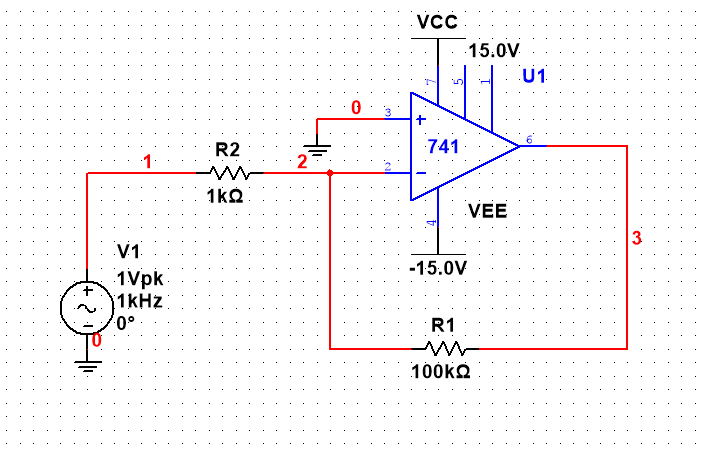
\includegraphics[width=10cm]{Task2-1-Circuit}\\
    \captionof{figure}{The circuit in task 2.1}    
    \end{minipage}\\
\pagebreak 


  \begin{minipage}{\linewidth}
  \centering
      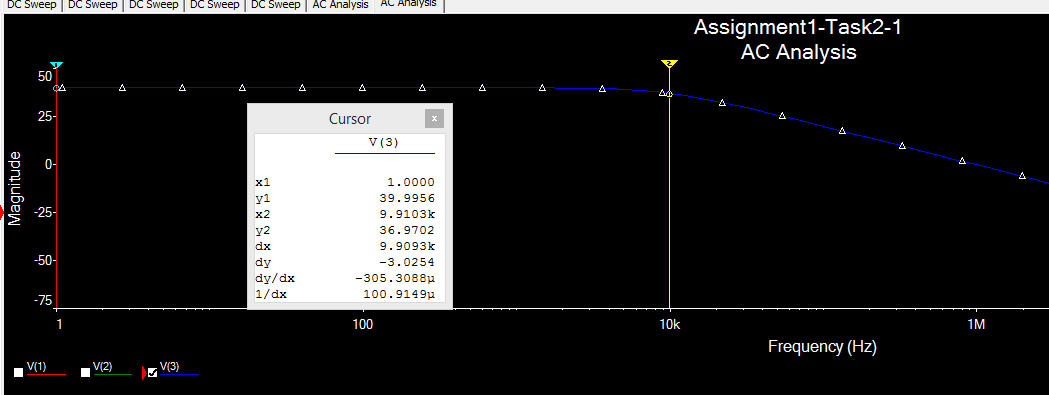
\includegraphics[width=14cm]{Task2-1-ACAnalysis}\\
    \captionof{figure}{AC analysis of the circuit shown in figure 8}    
    \end{minipage}\\
    
Figure 9 shows the AC analysis and from it the 3dB  frequency is found.
$$ f_{3dB} = 9.910 \ kHz $$

  \item[2.]
  By using the theoretical values to compare the to simulated result of the 3 dB frequency.
$$f_{t} = A_{t}f_{b}$$
$$ f_{b} = \frac{f_{t}}{A_{b}} = \frac{1\ MHz}{100 \frac{V}{V}} = 10\ kHz $$
The theoretical value is close to the simulated value from the AC analysis.  

\end{enumerate}
\pagebreak
\section*{Task 3: Op Amplifies Design}

\begin{enumerate}
  \item[1.]
  An op-amp-based integrator was designed with the DC gain equal to -10 V/V where \\R$_1$ = 200$\Omega$ and R$_2$ = 2k$\Omega$ as can be seen in figure 10. The value of the capacitance C of the integrator was calculated so that its 3dB frequency is 50kHz. %Knowing the gain bandwith product of the $\mu$A741 op amp to be 1MHz the capacitance can be calculated with the following formula.
$$\omega_0 = \frac{1}{C\cdot R_2} \Leftrightarrow C = \frac{1}{\omega_0 \cdot R_2} \Leftrightarrow C  = \frac{1}{50\text{kHz}\cdot 2\pi \cdot 2k\Omega} = 1.592 nF $$
  \begin{minipage}{\linewidth}
    	\centering       
        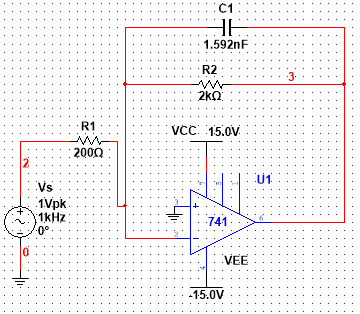
\includegraphics[width=7cm]{Task3_1.png}
        \captionof{figure}{Circuit diagram of an op-amp-based integrator} 
    \end{minipage}
  \item[2.]
  Simulation of the integrator seen in figure 11, shows that the 3dB frequency is 33.8kHz. This is not as predicted by theory from task 3.1. Previous calculations were done assuming an ideal amplifier which is not correct. There is a significant difference between the result and the expected result so further analysis must be done in order to find the correct value of the capacitance C so that the 3 dB frequency will be 50 kHz.\\
  \begin{minipage}{\linewidth}
    	\centering       
        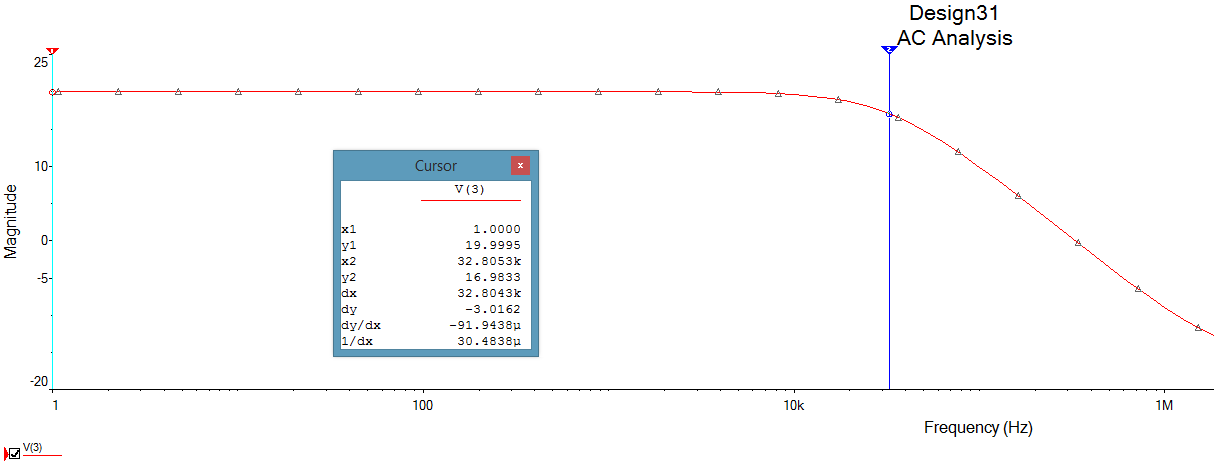
\includegraphics[width=14cm]{Task3_2.png}
        \captionof{figure}{AC analysis of the op-amp-based integrator with C = 1.592nF. } 
    \end{minipage} 
    \pagebreak
  \item[3.]
  The capacitance was determined again by neglecting the finite GBW. Assuming that the gain will reach zero dB, the transfer function is equal to one since log(1) = 0 dB. 
  $$| \frac{V_o(j\omega)}{V_i(j\omega)} | = | \frac{\frac{R_2}{R_1}}{1+j\omega \cdot C \cdot R_2} | = \frac{\frac{2k\Omega}{200\Omega}}{\sqrt{1^2+(10^6 \cdot 2\pi \cdot C \cdot 2k\Omega)^2}} = 1$$
  $$\Leftrightarrow C = \sqrt{\frac{\frac{R_2}{R_1}^2-1}{(\omega \cdot R_2)^2}}  = \sqrt{\frac{10^2-1}{(10^6 \cdot 2\pi \cdot 2k\Omega)^2}} = 0.792nF$$
  
By performing the AC analysis as in task 3.1 the 3dB frequency is found to be 48.66kHz as shown in figure 12.\\
\begin{minipage}{\linewidth}
    	\centering       
        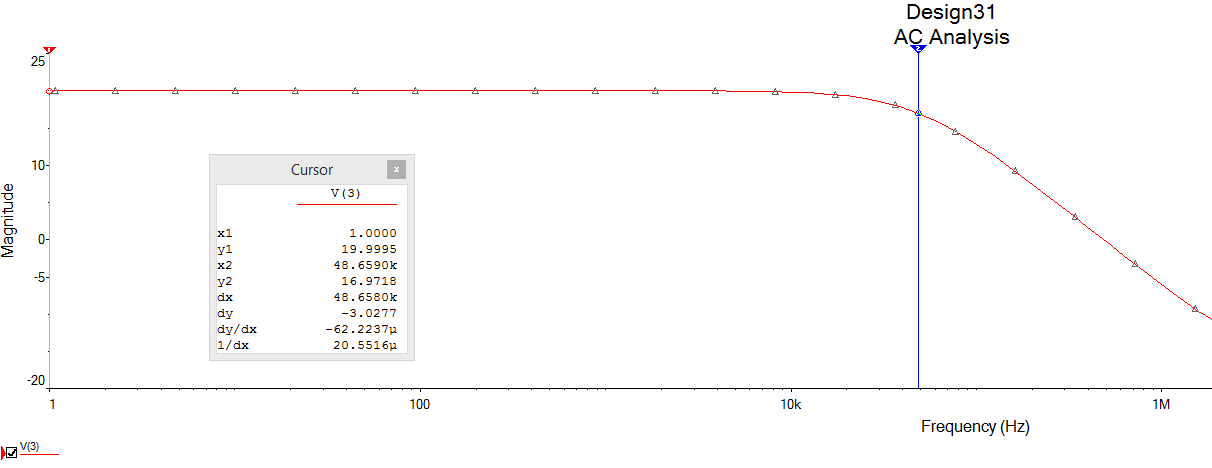
\includegraphics[width=14cm]{Task3_3.png}
        \captionof{figure}{AC analysis of the op-amp-based integrator with C = 0.792nF. } 
    \end{minipage}
\end{enumerate}



\pagebreak
\section*{Task 4: Half - Wave Rectifier}

\begin{enumerate}
  \item[$\bold{1.}$]
  A half-wave rectifier circuit was designed in $MultiSim$ as seen in figure 13:
  \\
  
	\begin{minipage}{\linewidth}
    	\centering
        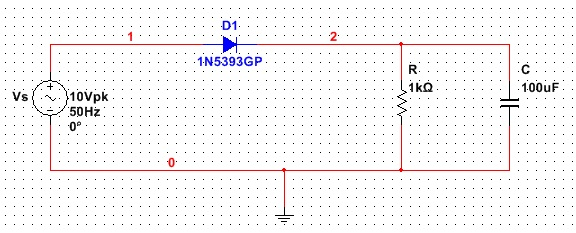
\includegraphics[width=13cm]{4_1.jpg}
        \captionof{figure}{The circuit in task 4.1}  
    \end{minipage}
    
  
  \item[$\bold{2.}$]
 	A transient analysis of the circuit was performed and the values of the peak and ripple voltages were found:
  \\
	\begin{minipage}{\linewidth}
    	\centering
        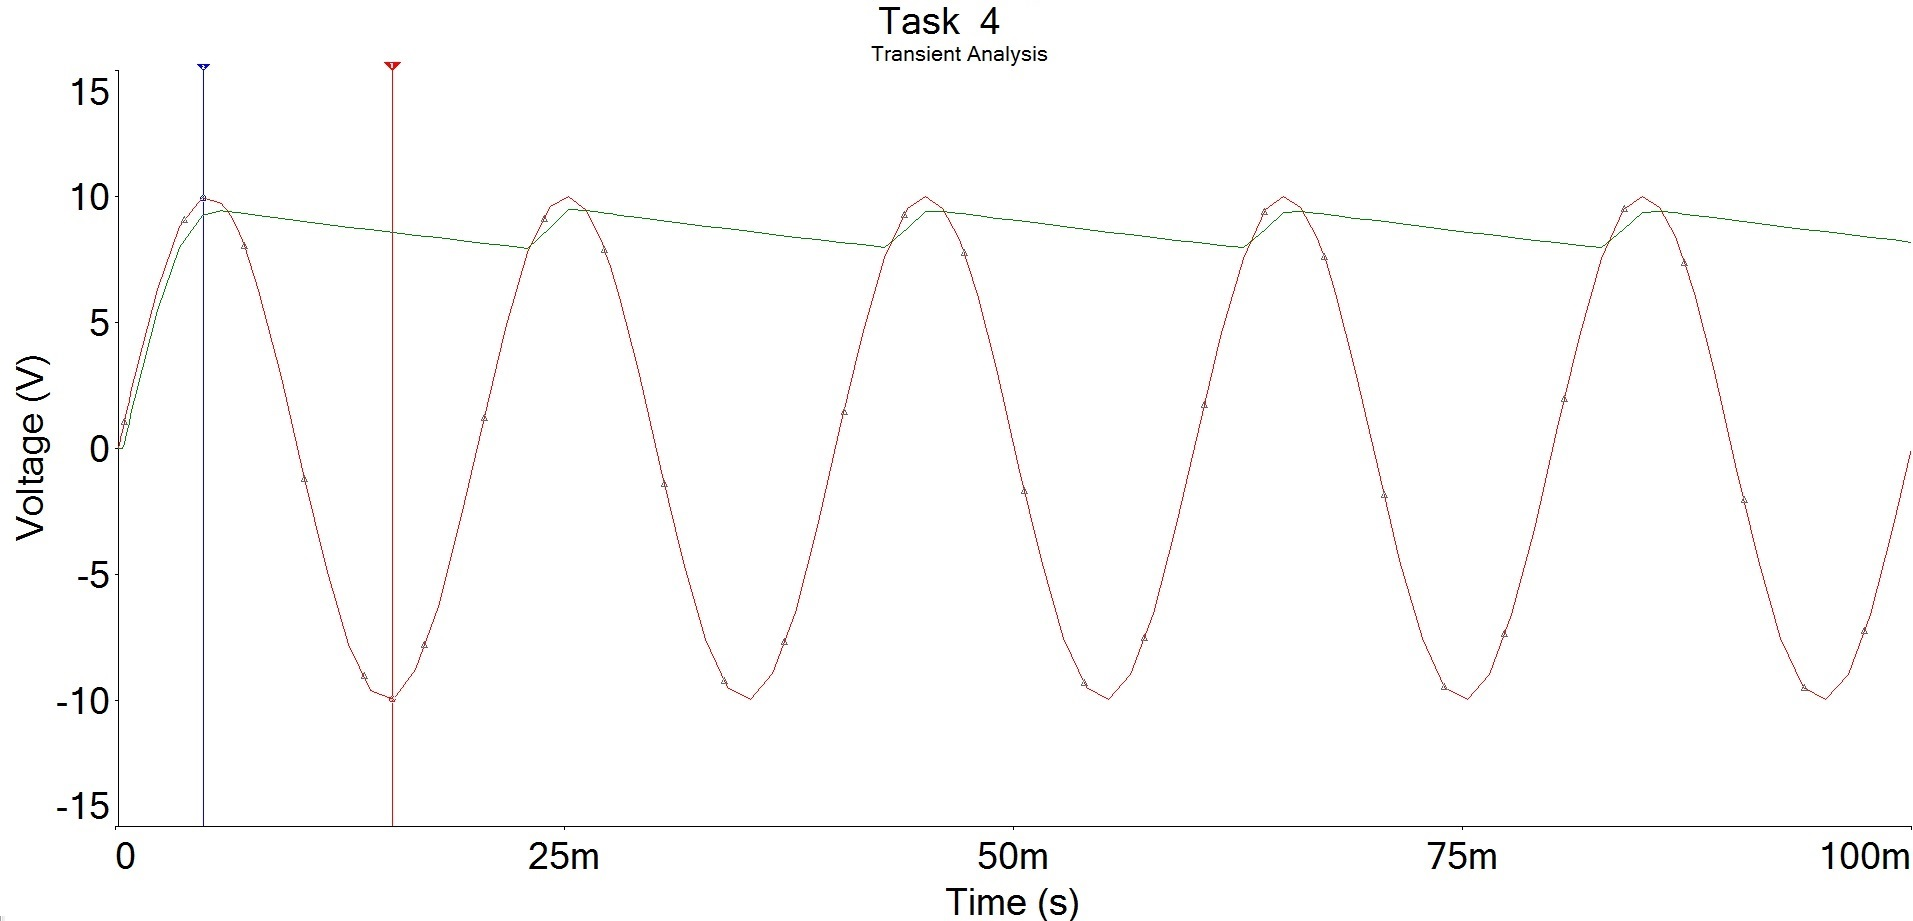
\includegraphics[width=13cm]{4_2.jpg}
        \captionof{figure}{Transient analysis the circuit in figure 13}  
    \end{minipage}

    \pagebreak
    
    
    \begin{minipage}{\linewidth}
    	\centering
        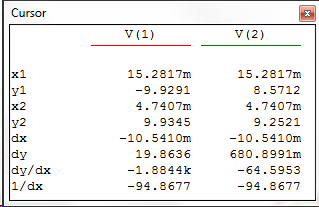
\includegraphics[width=9cm]{table_4_1.png}
        \captionof{figure}{The data for the cursors from figure 14}
    \end{minipage}
    
    \vspace{2em}
        
    The peak voltage is represented by y2 in figure 15, $V_p = 9.935 \ V$ 
    
    The theoretical value of $V_p$ is defined as the input voltage $V_s = 10 \ V$. The actual value of $V_p$ is close to the theoretical but the difference is caused by a small voltage drop in the diode used in $MultiSim$. \\
    
    \begin{minipage}{\linewidth}
    	\centering
        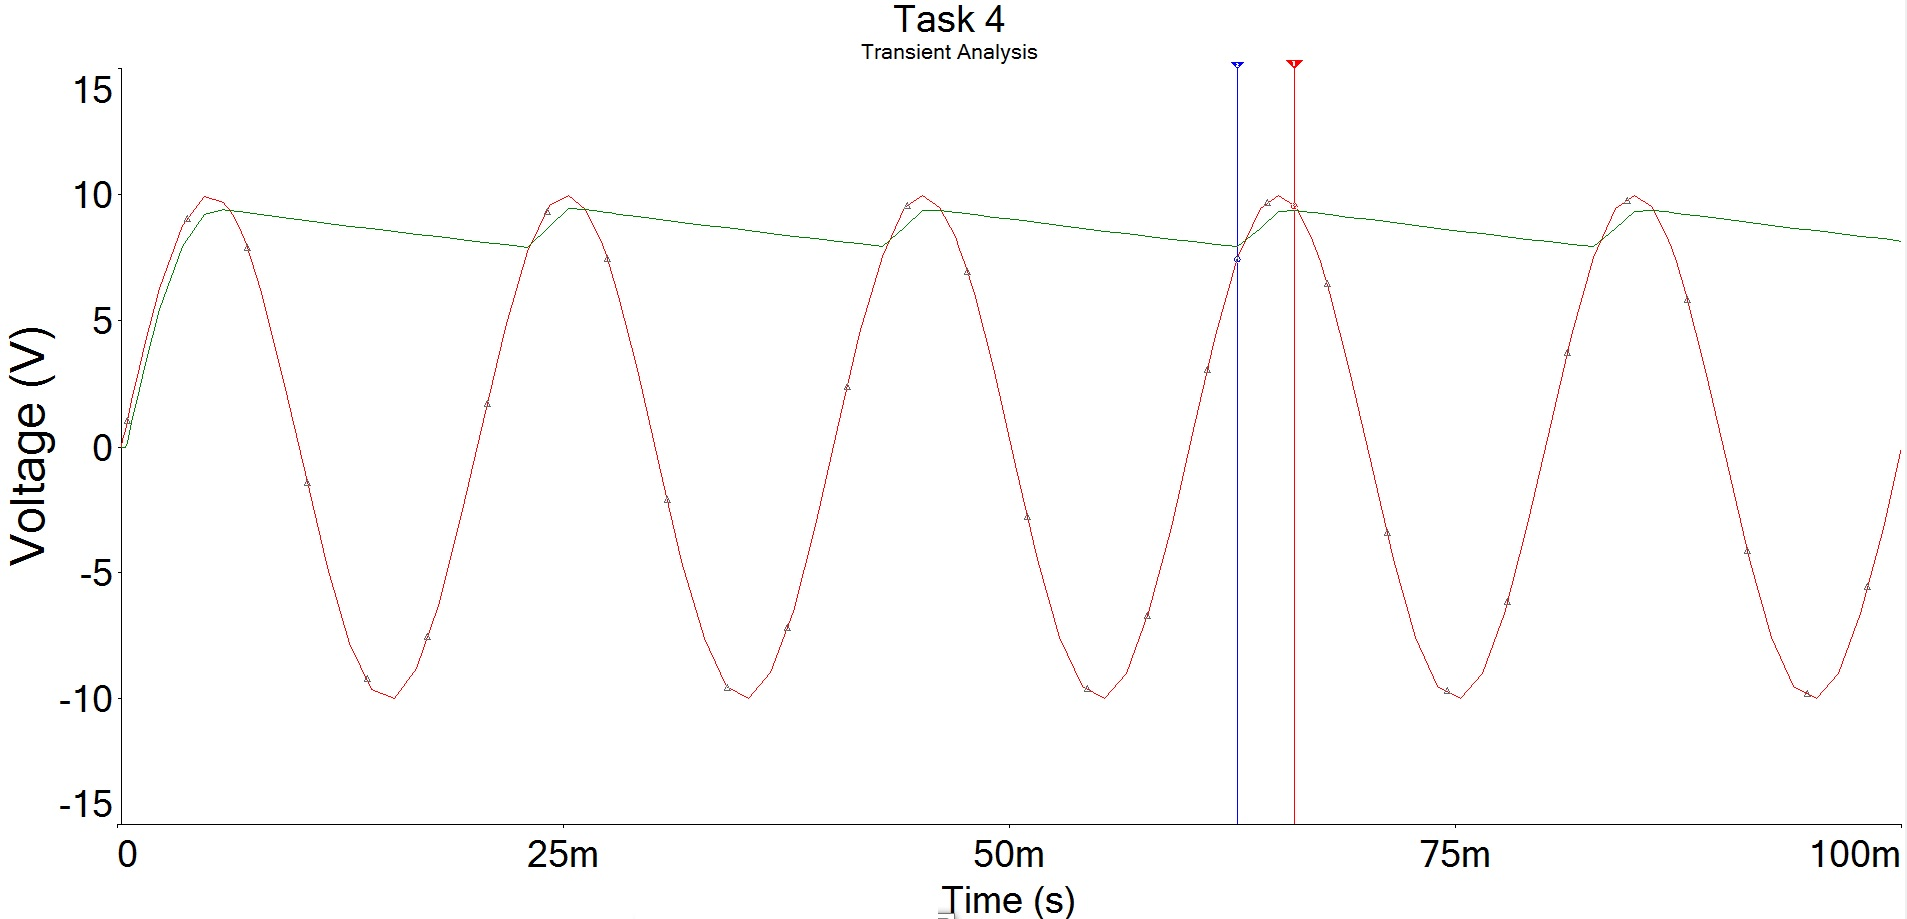
\includegraphics[width=13cm]{4_3.jpg}
        \captionof{figure}{The voltage difference over one period, measured for the circuit in figure 13 } 
    \end{minipage}
    
    \begin{minipage}{\linewidth}
    	\centering
        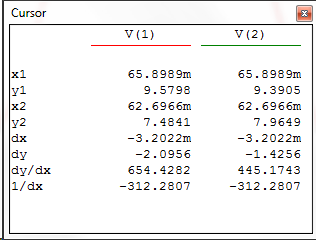
\includegraphics[width=9cm]{table_4_2.png}
        \captionof{figure}{Data from the cursor in figure 16}
    \end{minipage}
    
    \vspace{2em}
    
	The ripple voltage can be calculated from figure 16 and the data in figure 17. The maximum difference in voltage over the diode over one period is the ripple voltage hence it can be seen from the graph and table by using the cursors (figure 16 and 17): $$ V_r = 9.5798\ V - 7.4841 \ V = 2.096 \ V$$
    The theoretical ripple voltage value can then be calculated: $$ V_r = \dfrac{V_p}{fCR} = \dfrac{10}{50 \cdot 100 \cdot 10^{-6} \cdot 10^3} = 2\ V$$
  
  \item[$\bold{3.}$]
  
  	The ripple voltage will then be: $V_r(max) = V_p \cdot 0.02 = 0.1987\ V$. Hence the maximum value of the capacitance can calculate: $$ C = \dfrac{V_p}{f R V_r} = \dfrac{V_p}{f R V_p \cdot 0.02} = \dfrac{1}{f R \cdot 0.02} = \dfrac{1}{50 \cdot 10^3 \cdot 0.02} = 1mF $$
  	
  	\begin{minipage}{\linewidth}
    	\centering
        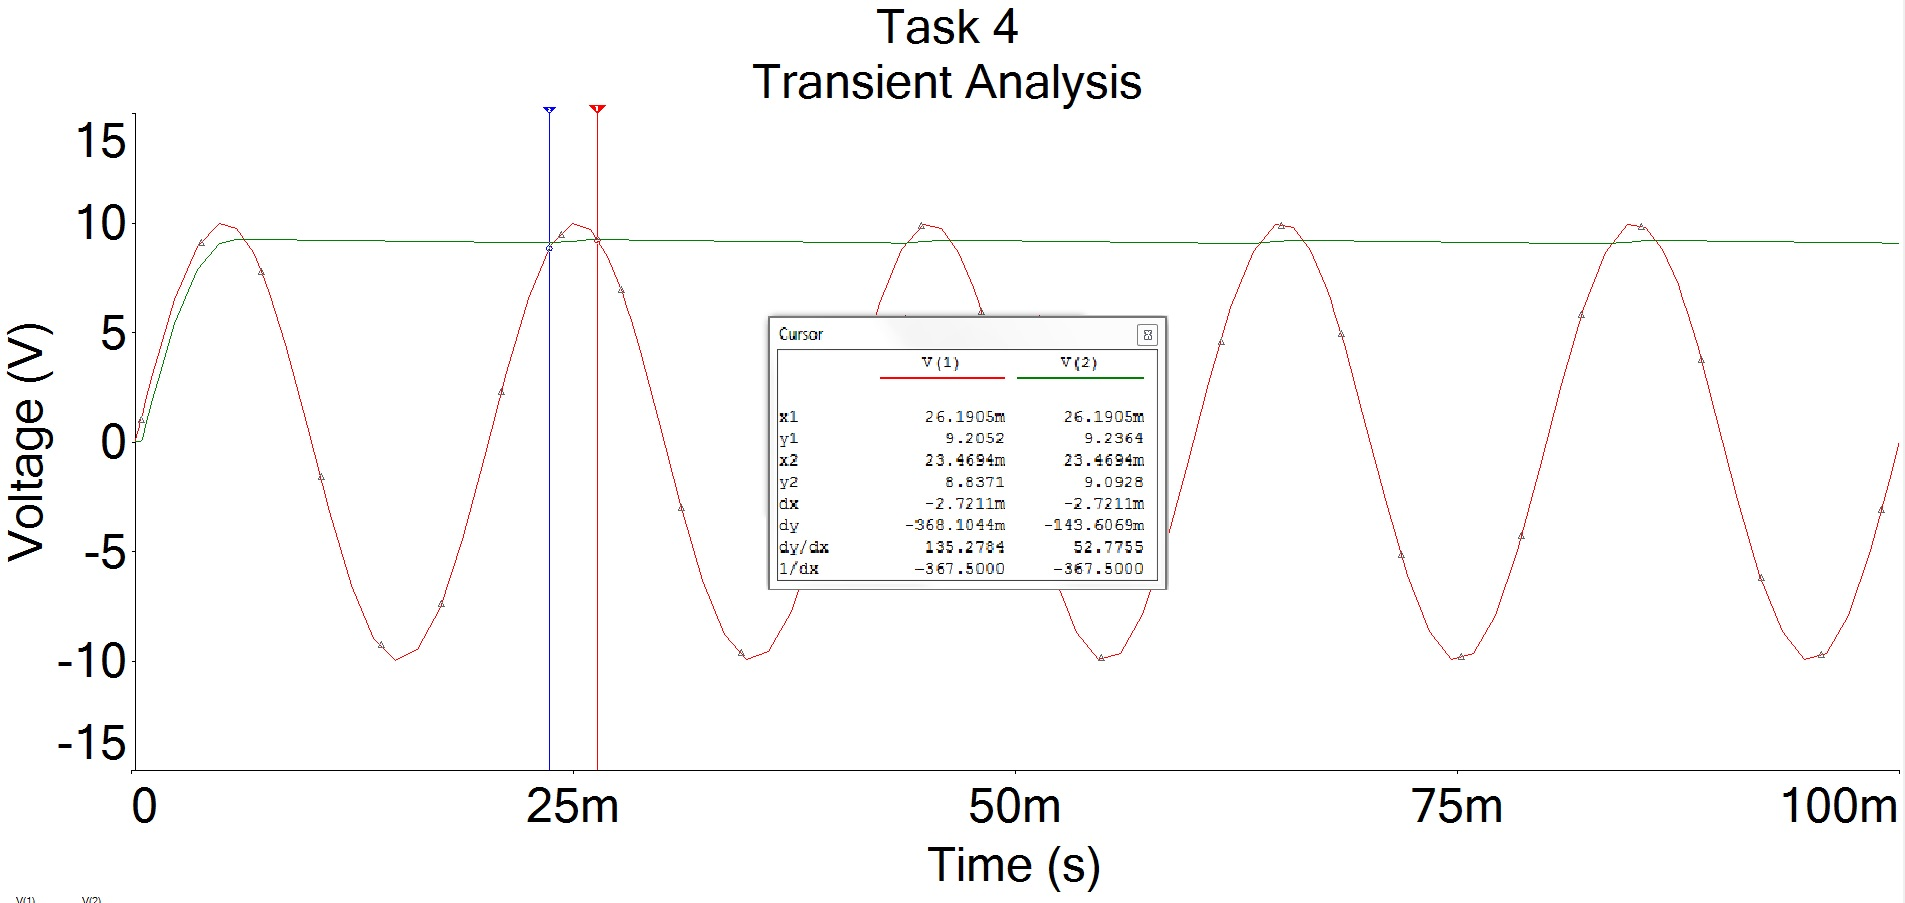
\includegraphics[width=15cm]{4_4.jpg}
        \captionof{figure}{The value of capacitor has been changed to $1mF$ as calculated}
    \end{minipage}
    \vspace{1em}
    
   From the table in figure 18: $$ V_r = 9.2364 \: V- 9.0928\: V = 0.1436\: V < V_r(max) = 0.1987\: V$$ 
    So the analysis holds and the ripple voltage from the analysis is smaller then the maximum value.
  
\end{enumerate}

  


\end{document}
\\
